\subsection{Fibonacci sequence}

You have just received a birthday present. It's a pair of rabbits from the
Neverdie Island.
Let's call this pair of rabbits $P_1$.
At the end of the first month, nothing happens -- you still have $P_1$.
Then suddenly at the end of the second month,
the pair $P_1$ produces a pair of male and
female baby rabbits $P_{11}$.

You see, every pair of male and female rabbits from Neverdie Island will
start producing
a pair of male and female rabbits after 2 months and continue to do so
every month.

At the beginning there's 1 pair.
After one month, there's still 1 pair (the same $P_1$).
After two months, there are 2 pairs -- there's $P_1$ and the offspring pair
$P_{11}$ of $P_1$.
After 3 months, there are 3 pairs -- there's $P_1$ and first offspring pair
$P_{11}$
and the new pair $P_{12}$. Note that $P_{11}$ don't have offsprings yet.
The following diagram might be more systematic:
  
\begin{python}
from latextool_basic import *
from latexcircuit import *
p = Plot()
Graph.r = 0.4
Graph.background='blue!5'
d = positions('''
A
B
C               D
E         F     G
H     J   T     U     6
I   K N   S   2 V   0 5
L M O P Q R 1 3 W X Y Z 4
''', xscale=0.55)

label = {'A':'$P_1$',
         'B':'$P_1$',
         'C':'$P_1$',
         'D':'$P_{11}$',
         'E':'$P_1$',
         'F':'$P_{12}$',
         'G':'$P_{11}$',
         'H':'$P_1$',
         'I':'$P_1$',
         'J':'$P_{13}$',
         'K':'$P_{14}$',
         'L':'$P_{1}$',
         'M':'$P_{15}$',
         'O':'$P_{14}$',
         'N':'$P_{13}$',
         'P':'$P_{13}$',
         'Q':'$P_{131}$',
         'R':'$P_{12}$',
         'S':'$P_{12}$',
         'T':'$P_{12}$',
         'U':'$P_{11}$',
         'V':'$P_{11}$',
         'W':'$P_{11}$',
         'X':'$P_{113}$',
         'Y':'$P_{112}$',
         'Z':'$P_{111}$',
         '0':'$P_{112}$',
         '1':'$P_{122}$',
         '2':'$P_{121}$',
         '3':'$P_{121}$',
         '4':'$P_{1111}$',
         '5':'$P_{111}$',
         '6':'$P_{111}$',
}
for k in label:
    label[k] = r'{\scriptsize %s}' % label[k]

edges = ['CD', 'HJ', 'IK', 'EF', 'LM', 'HJ', 'PQ', 'Z4', 'S2', 'R1', 'WX', 'V0', 'U6']
    
for k in d:
    x,y = d[k]
    lab = label[k]
    p += Graph.node(x=x, y=y, label=lab, name=k)
    
for e in edges:
    k0,k1 = e
    p += Graph.arc(names=[k0,k1])
    
x,y = d['A']
X = POINT(x=x+14, y=y, r=0, label=r'{\scriptsize beginning}')
p += str(X)

x,y = d['B']
X = POINT(x=x+14, y=y, r=0, label=r'{\scriptsize after 1 month}')
p += str(X)

x,y = d['C']
X = POINT(x=x+14, y=y, r=0, label=r'{\scriptsize after 2 months}')
p += str(X)

x,y = d['E']
X = POINT(x=x+14, y=y, r=0, label=r'{\scriptsize after 3 months}')
p += str(X)

for xs in ['FTSR', 'KO', 'ABCEHIL', 'JNP', '23', 'DGUVW', '0Y', '65Z']:
    xs = list(xs)
    xs = zip(xs[:-1], xs[1:])
    for e in xs:
        k0,k1 = e
        p += Graph.edge(names=[k0,k1])
        
print(p)
\end{python}
      
The number of pairs at the beginning and at the end of each
month give rise to the following sequence
\[
1,1,2,3,5,8,13,...
\]
This is called the \defone{Fibonacci sequence}.
Let $F_n$ be the number of pairs after $n$ month.
Then $F_0 = 1, F_1 = 1, F_2 = 2, F_3 = 3, F_4 = 5, F_5 = 8, ...$.

The question is this:
How many pairs of rabbits do you have at the end of 12 months?
Continuing the above \lq\lq accounting" diagram is painful.
So ... show that
\[
F_n = F_{n - 1} + F_{n - 2}
\]
if $n \geq 2$.
And then compute $F_{12}$.
(This problem appeared in the book
\href{https://en.wikipedia.org/wiki/Liber_Abaci}{Liber Abaci}
written by \href{https://en.wikipedia.org/wiki/Fibonacci}{Fibonacci} in 1202.) 

(Hint: It's basic accounting. You want to keep track of which
pair can reproduce.
So I suggest you keep track of the ages of the pairs.
Spoiler (hint) on next page ...)

\newpage
WARNING ... INCOMING SPOILER ...

\textsc{Hint.}

You might want to keep track on the number of pairs of rabbits for
three age groups: just born, one year old, at least two years old.

Spoiler (solution) on next page ...

\newpage
WARNING ... INCOMING SPOILER ...

\textsc{Solution.}

Our goal is to prove $F_n = F_{n-1} + F_{n-2}$.

The proof is derived by basically keeping track of numbers (i.e. accounting).
At time $n$, I have $F_n$ pairs.
I want to count the number of pairs
$F_{n+1}$ (number of pairs at time $n + 1$) and also at time $n + 2$.
The number of pairs at time $n + 1$ (and also $n + 2$) depends on
how many pairs can reproduce (right?). So I break up my pairs at time $n$
by age:
\begin{Verbatim}[fontsize=\footnotesize]
  Fn   = A (age 0) + B (age 1) + C (age >= 2) 
\end{Verbatim}
where there are $A$ pairs of age 0, $B$ pairs of age 1, $C$ pairs at age 2 and
older.
What happens at time $n + 1$? I have this:
\begin{Verbatim}[fontsize=\footnotesize]
  Fn   = A (age 0) + B (age 1)             + C (age >= 2)
         |           |                       |
         |           +-----------+           +-------------+
         |           |           |           |             |
  Fn+1 = A (age 1) + B (age 2) + B (age 0) + C (age >=2) + C (age=0)
  \end{Verbatim}
Correct? I'll let you do some basic accounting check on the above.
Reorganizing by age groups, I get this:
\begin{Verbatim}[fontsize=\footnotesize]
  Fn   = A (age 0) + B (age 1) + C (age >= 2)
  Fn+1 = A (age 1) + B (age 2) + B (age 0) + C (age >=2) + C (age=0)
       = (B + C) (age 0) + A (age 1) + (B + C) (age >= 2)
  \end{Verbatim}
OK. Now what happens at time $n + 2$? I get this:
\begin{Verbatim}[fontsize=\footnotesize]
  Fn   = A (age 0) + B (age 1) + C (age >= 2)
  Fn+1 = A (age 1) + B (age 2) + B (age 0) + C (age >=2) + C (age=0)
       = (B + C) (age 0) + A (age 1)             + (B + C) (age >= 2)
         |                 |                       |
         |                 +-----------+           +-------------------+
         |                 |           |           |                   |
  Fn+2 = (B + C) (age 1)   A (age 2) + A (age 0)   (B + C) (age >= 2)  (B + C) (age = 0)
\end{Verbatim}
Yes? Reorganizing, I get this
\begin{Verbatim}[fontsize=\footnotesize]
  Fn   = A (age 0) + B (age 1) + C (age >= 2)
  Fn+1 = A (age 1) + B (age 2) + B (age 0) + C (age >=2) + C (age=0)
       = (B + C) (age 0) + A (age 1) + (B + C) (age >= 2)
  Fn+2 = (B + C) (age 1) + A (age 2) + A (age 0) + (B + C) (age >= 2)  (B + C) (age = 0)
       = (A + B + C) (age 0) + (B + C) (age 1) + (A + B + C) (age >= 2)
  \end{Verbatim}
Ignoring the age data, I have this:
\begin{align*}
  F_n &= A + B + C \\
  F_{n+1} &= B + C + A + B + C = A + 2(B + C)\\
  F_{n+2} &= A + B + C + B + C + A + B + C = 2A + 3(B + C)
\end{align*}
Therefore
\[
F_n + F_{n + 1} = \left(A + B + C\right) + \left(A + 2(B + C)\right) = 2A + 3(B + C) = F_{n + 2}
\]
Voil\`a! QED.
\qed

The above notation
\begin{Verbatim}[fontsize=\footnotesize]
  Fn   = A (age 0) + B (age 1) + C (age >= 2)
  Fn+1 = A (age 1) + B (age 2) + B (age 0) + C (age >=2) + C (age=0)
       = (B + C) (age 0) + A (age 1) + (B + C) (age >= 2)
  Fn+2 = (B + C) (age 1) + A (age 2) + A (age 0) + (B + C) (age >= 2)  (B + C) (age = 0)
       = (A + B + C) (age 0) + (B + C) (age 1) + (A + B + C) (age >= 2)
  \end{Verbatim}
is not very mathematical, hard to read, and messy.

To use proper mathematical notation, I will rewrite the above
using a 3-tuple $(A, B, C)$
to describe the number of pairs of age 0, age 1, and age $\geq 2$.
Let $G_n$ be the 3-tuple of pairs at time $n$.
For instance $G_0 = (1, 0, 0)$, $G_1 = (0, 1, 0)$, and $G_2 = (1, 0, 1)$.
You then get this:
\[
\text{if } G_n = (A, B, C), \text{ then }
G_{n+1} = (B + C, A, B + C)
\]
And now applying this fact to $G_{n + 1}$, you get
\begin{align*}
G_{n+1} = (B + C, A, B + C) \implies
G_{n + 2} &= (A + (B + C), B + C, A + (B + C)) \\
         &= (A + B + C, B + C, A + B + C)
\end{align*}
Clearly the relation between $F_n$ and $G_n$ is
\[
\text{if } G_n = (A,B,C), \text{ then } F_n = A + B + C
\]
and you'll arrive at pretty much the same proof before
but using a cleaner and a more mathematical presentation.
Now write up a proper proof using \LaTeX.

Cleanness and clarity is important for both math and writing code.

%\newpage

\begin{ex} 
  \label{ex:some-decision1}
  \tinysidebar{\debug{exercises/{empty0/question.tex}}}
  \solutionlink{sol:some-decision1}
  \qed
\end{ex} 
\begin{python0}
from solutions import *
add(label="ex:some-decision1",
    srcfilename='exercises/some-decision1/answer.tex') 
\end{python0}

%\newpage

\begin{ex} 
  \label{ex:some-decision1}
  \tinysidebar{\debug{exercises/{empty0/question.tex}}}
  \solutionlink{sol:some-decision1}
  \qed
\end{ex} 
\begin{python0}
from solutions import *
add(label="ex:some-decision1",
    srcfilename='exercises/some-decision1/answer.tex') 
\end{python0}

%\newpage

\begin{ex} 
  \label{ex:some-decision1}
  \tinysidebar{\debug{exercises/{empty0/question.tex}}}
  \solutionlink{sol:some-decision1}
  \qed
\end{ex} 
\begin{python0}
from solutions import *
add(label="ex:some-decision1",
    srcfilename='exercises/some-decision1/answer.tex') 
\end{python0}




\begin{comment}
0:    1, 0, 0, 0, ..., 0
1:    0, 1, 0, 0, ..., 0
2:    0, 0, 1, 0, ..., 0


b:    a, 0, 0, 0, ..., 1
b+1:  a, a, 0, 0, ..., 1
b+2:  a, a, a, 0, ..., 1

2b:   a+a^2, a, a, a, ..., 1+a
2b+1:

3b:   a+a^2+a^2+a^3
\end{comment}
\begin{comment}
In fact if you define the function $g(a, b, c) = (b + c, a b + c)$,
and the function $\operatorname{sum}(a, b, c) = a + b + c)$,
you'll see that the Fibonacci recurrence relation is the same as saying
\[
\operatorname{sum}(g(g(a,b,c))) = \operatorname{sum}(a,b,c) + \operatorname{sum}(g(a,b,c)) 
\]
Looking at the function $g$ again:
\[
g(a, b, c) = (b + c, a, b + c)
\]
you can view the input as a 3-dimensional vector:
\[
g
\left(
\begin{bmatrix}
  a \\
  b \\
  c
\end{bmatrix}
\right)
=  
\begin{bmatrix}
  b + c \\
  a \\
  b + c
\end{bmatrix}
=
\begin{bmatrix}
  0 & 1 & 1 \\
  1 & 0 & 0 \\
  0 & 1 & 1
\end{bmatrix}
\begin{bmatrix}
  a \\
  b \\
  c
\end{bmatrix}
\]
Initially $a=1, b=0, c=0$.
Of course for $F_n$, you will need to compute
\[
\begin{bmatrix}
  0 & 1 & 1 \\
  1 & 0 & 0 \\
  0 & 1 & 1
\end{bmatrix}^n
\begin{bmatrix}
  1 \\
  0 \\
  0
\end{bmatrix}
\]
This gives the three components of $F_n$.
\[
\begin{bmatrix}
  0 & 1 & 1 \\
  1 & 0 & 0 \\
  0 & 1 & 1
\end{bmatrix}
=
P
\begin{bmatrix}
  0 & 1 & 1 \\
  1 & 0 & 0 \\
  0 & 1 & 1
\end{bmatrix}
\begin{bmatrix}
  \varphi' & 0       & 0 \\
  0        & \varphi & 0 \\
  0        & 0       & 0
\end{bmatrix}
P^{-1}
\]
where
\[
P =
\begin{bmatrix}
  1        & 1       & 0 \\
  -\varphi & \varphi & 0 \\
  1        & 1 & 1
\end{bmatrix}
\]
\end{comment}

%\newpage
CS, math, physics, engineering is heavily involved
in the analysis of functions. (Right?)
For instance I can ask
\lq\lq if an object mass $m$ and starts moving on a straight line
at velocity $v$,
where is it at time $t$?" Here I am asking for the position function
$p(t)$, where $t \in \R$.
In the case of the Fibonacci sequence, the function is $F(n)$ (or $F_n$) where
$n \in \N$.
A function with a domain of $\{0,1,2,...\}$ is very common in CS, engineering, and math.
So a sequence of numbers is really just a function with domain $\{0,1,2,...\}$.

Frequently, the sequence of numbers we want to 
study actually obey a recurrence relation.
What do I mean?
Well take for instance the famous Fibonacci sequence
\[
1, 1, 2, 3, 5, \ldots
\]
Now by definition if we denote the sequence by $F_n$, we see that
\[
F_n = F_{n-1} + F_{n-2}
\]
for $n \geq 2$.
Once two base conditions are given, the $F_n$'s are well-defined.

In general,
given a sequence $a_0, a_1, a_2, ...$ (or equivalently a function with domain $\{0, 1, 2, ...\}$),
a \defone{recurrence relation} is an algebraic expression of $a_n$ in terms of
$n, a_0, ..., a_{n-1}$
whenever $n \geq d$ for some $d \geq 0$.
The values for $a_0, ..., a_{d-1}$ are called
\defone{base cases/conditions}.

For our $F_n$'s, 
I'm going to change the first two numbers from $1,1$ to $0,1$:
\[
F_n
=
\begin{cases}
0 &\text{ if } n = 0 \\
1 &\text{ if } n = 1 \\
F_{n-1} + F_{n-2}  &\text{ if } n \geq 2 \\
\end{cases}
\]
Instead of the sequence
\[
1, 1, 2, 3, 5, 8, 13, ...
\]
The sequence is now
\[
0, 1, 1, 2, 3, 5, 8, ...
\]

Here are a few more recurrence relations:
\begin{align*}
  a_n &= 2a_{n - 3} \\
  b_n &= 3b_{n - 3} + 4b_{n - 7} \\
  c_n &= c_{n - 3} + 7c_{n - 7} + n^2\\
  d_n &= d_{n - 3} d_{n-4} \\
  e_n &= 42e_{n - 3} + e_{n-4}^2\\
  f_n &= f_{n - 1} \sqrt{f_{n-2} + f_{n-3}}\\
  g_n &= g_{\floor{n/2}} + n \\
  h_n &= \frac{1}{n} \sum_{k=0}^{n-1} h_k \\
  j_n &= j_{n-1}j_0 + j_{n-2}j_1 + j_{n-3}j_2 + \cdots + j_1j_{n-2} + j_0j_{n-1}
\end{align*}
Of course you can also write the numbers in a sequence using
function notation.
So instead of writing $F_n$, sometimes I can also write
$F(n)$.
This is especially the case when the subscripts/indexes are complex such as
\[
  g_n = g_{\floor{n/2}} + n
\]
which will sometimes be written
\[
  g(n) = g(\floor{n/2}) + n
\]
or say something more complex like
\[
  g(n) = g(n - \floor{n/2}) + n
\]
Otherwise you'll have to squint your eyes at the subscripts:
\[
  g_n = g_{n - \floor{n/2}} + n
\]

Suppose a problem gives rise to a sequence $a_n$
(or function with domain of $\{0,1,2,...\}$). 
Frequently you want a way to be able to compute $a_n$ when given a value for
$n$.
For instance in the Fibonacci problem, you want $F_{12}$.

A recurrence relation on $a_n$, if found, will let you compute $a_n$
for any $n$ using the recurrence relation, but usually this is very slow
(see CISS350).
In the case of computing $F_{n}$ (the $n$--th Fibonacci number) using
the Fibonacci recurrence relation, the time taken (the runtime)
is exponential!
For instance it would be impossible for you to compute $F_{60}$ by hand or by
using your laptop. (Do ahead and try it.)
So $F_{12}$ is very tedious (but the recurrence relation is still better
than drawing pictures to do rabbit accounting).

To speed up the computation, one way would be to find a closed form for $a_n$,
i.e., a formula for $a_n$ in terms of $n$.
Just like 
\[
s_n = 1 + 2 + \ldots + n
\]
is quickly evaluated using the closed-form 
\[
s_n = \frac{n(n+1)}{2}
\]
A \defone{closed form} for a sequence $a_0, a_1, a_2, ...$ is a formula
for $a_n$ in terms of $n$ (and not $a_i$'s).
Sometimes the formula might not apply to the first few terms of
the sequence (the base cases). 

Not only that:
a closed-form is also easier to use for approximation,
especially in the case of asymptotic approximations.
For instance
\[
s_n = \frac{n(n+1)}{2}
\]
is asymptotically bounded above by $n^2$, i.e.
\[
s_n = \frac{n(n+1)}{2} = O(n^2)
\]
This is the situation where you want to compare the growth of two
functions for large $n$ and you are not interested in 
specific values such as $s_{1000}$.

If you have a recurrence for a sequence, there are techniques to
compute a closed form, or if that fails, one can try to
compute approximations, or if that also fails, then one can try to
compute asymptotic approximations:

\begin{python}
from latextool_basic import *
p = Plot()
p += Rect(x0=0, y0=0, x1=3, y1=1, label='problem', name='problem')
p += Rect(x0=4, y0=0, x1=8, y1=1, label='recurrence relation', name='recurrence')
p += Rect(x0=9, y0=0, x1=13, y1=1, label='closed form', name='closed form')
p += Line(names=['problem', 'recurrence'], linecolor='blue', endstyle='>')
p += Line(names=['recurrence', 'closed form'], linecolor='blue', endstyle='>')
p += Line(names=['problem', 'closed form'], bend_right='20', linecolor='red', endstyle='>')
print(p)
\end{python}

Although the ultimate goal is the closed form, frequently the
intermediate step of finding recurrence relation cannot be avoided.
In fact it's a crucial step.

We say that the Fibonacci sequence
$F_n$ satisfies a \defone{degree} 2 recurrence relation.
The \lq\lq 2" is due to the fact that in the recurrence relation
\[
F_n = F_{n-1} + F_{n-2} \\
\]
if you look at the subscripts/indices:
\[
F_{\text{\textbox{$n$}}} = F_{\text{\textbox{$n - 1$}}} + F_{\text{\textbox{$n - 2$}}} 
\]
i.e.,
\[
n, \,\,\, n-1, \,\,\, n-2
\]
the maximum absolute difference is 2.
In general $a_0, a_1, ...$ is a \defone{degree} $k$ relation if there is a
formula ${\mathcal F}(x_0, ..., x_{k})$ such that
\[
{\mathcal F}(a_{n-k}, ..., a_{n}) = 0
\]
In the case of the Fibonacci recurrence relation,
the formula is
\[
  {\mathcal F}(x_0, x_1, x_2) = x_2 - x_1 - x_0
  \]
since if you
substitute
$x_2$ by $F_n$, 
$x_1$ by $F_{n-1}$, 
$x_0$ by $F_{n-2}$,
you get
\[
  {\mathcal F}(F_{n-2}, F_{n-1}, F_{n}) = F_n - F_{n-1} - F_{n-2}
\]
and
\[
  {\mathcal F}(F_{n-2}, F_{n-1}, F_{n}) = 0
  \]
is exactly our Fibonacci recurrence relation
$F_n = F_{n-1} + F_{n-2}$.
It should be obvious that the higher the degree, the more complex
is the recurrence relation and the longer it will take
to compute a specific term of the sequence.

(\textsc{Aside}: Of course if 
$F_n = F_{n-1} + F_{n-2}$, then
it's also true that
$F_n = F_{n-1} + F_{n-2} + 0 \cdot F_{n-3}$, but you don't
consider terms like $0 \cdot F_{n-3}$ and say the Fibonacci
sequence has degree $3$! Please don't do that!)

Note that the worst case is where the computation of
$a_n$ depends on \textit{all} the previous $a_i$:
\[
a_n = \frac{1}{n} \sum_{i = 0}^{n-1} a_i
\]
and the degree is $n + 1$, i.e., the degree is not constant.
Here's an example where $b_n$ depends on half of the previous
$b_i$'s:
or at least the degree is not constant and grows with $n$:
\[
b_n = \sum_{i = 0}^{\floor{n/2}} b_i
\]
The degree is again not a constant.

In general a constant degree recurrence is easier to handle.
The cases of non-constant degree like the above are harder to
handle.
They are important because they occur in
\lq\lq average" computations (such as average runtime analysis).


\begin{ex} 
  \label{ex:some-decision1}
  \tinysidebar{\debug{exercises/{empty0/question.tex}}}
  \solutionlink{sol:some-decision1}
  \qed
\end{ex} 
\begin{python0}
from solutions import *
add(label="ex:some-decision1",
    srcfilename='exercises/some-decision1/answer.tex') 
\end{python0}


Furthermore we say that the Fibonacci recurrence relation is
linear.
It is a \defone{linear recurrence relation} because
$F_n, F_{n-1}$ and $F_{n-2}$
occurs as a sum of constant multiple (i.e. linear combination):
$F_{n} = F_{n-1} + F_{n-2}$ is the same as
\[
1 \cdot F_n - 1 \cdot F_{n-1} - 1 \cdot F_{n-2} = 0\\
\]
The following is also a linear recurrence (of degree 5):
\[
5 \cdot G_n = 7 \cdot G_{n-2} - 13 \cdot G_{n-5} \\
\]
However the following is nonlinear:
\[
a_n = n a_{n-1} - 3a_{n-2}
\]
because the coefficient in front of $a_{n-1}$ is $n$ which is not constant.
This is also not linear:
\[
a_n = a_{n-1}^2 - a_{n-2}
\]
because in front of $a_{n-1}$ is $a_{n-1}$ which is not a constant.
This is also not linear:
\[
a_n = \sqrt{a_{n-1}} - a_{n-2}
\]
because of $\sqrt{a_{n-1}}$.

%\newpage

\begin{ex} 
  \label{ex:some-decision1}
  \tinysidebar{\debug{exercises/{empty0/question.tex}}}
  \solutionlink{sol:some-decision1}
  \qed
\end{ex} 
\begin{python0}
from solutions import *
add(label="ex:some-decision1",
    srcfilename='exercises/some-decision1/answer.tex') 
\end{python0}

%\newpage

\begin{ex} 
  \label{ex:some-decision1}
  \tinysidebar{\debug{exercises/{empty0/question.tex}}}
  \solutionlink{sol:some-decision1}
  \qed
\end{ex} 
\begin{python0}
from solutions import *
add(label="ex:some-decision1",
    srcfilename='exercises/some-decision1/answer.tex') 
\end{python0}

%\newpage

\begin{ex} 
  \label{ex:some-decision1}
  \tinysidebar{\debug{exercises/{empty0/question.tex}}}
  \solutionlink{sol:some-decision1}
  \qed
\end{ex} 
\begin{python0}
from solutions import *
add(label="ex:some-decision1",
    srcfilename='exercises/some-decision1/answer.tex') 
\end{python0}



%\newpage
One of the most important type of nonlinear recurrences is of the form
\[
a(n) = a(\floor{n/2}) + 3n + 4
\]
or
\[
a(n) = 2a(\floor{n/2}) + 3n \lg n + 4
\]
or
\[
a(n) = a(\floor{n/2}) + a(n - \floor{n/2}) + n
\]
More generally such recurrences can be
\[
a(n) =  \alpha a(\floor{n/\beta}) + f(n)
\]
or
\[
a(n) =  \alpha_1 a(\floor{n/\beta}) + \alpha_2 a(n - \floor{n/\beta}) + f(n)
\]
where $\alpha, \alpha_i, \beta$ are constants and $f(n)$ is a formula in $n$.
These are called \defone{divide-and-conquer recurrences}.
In CS and engineering,
divide-and-conquer recurrences appear in the runtime analysis
of recursive algorithms
that involves the divide-and-conquer algorithm design technique.
These includes binary search, mergesort, quicksort, etc.

A recurrence relation in $a_0, a_1, a_2, ...$ is \defone{homogeneous} if
$a_n$ is expressed as a sum of expressions that involve some $a_i$.
For instance
\[
F_{n} = F_{n - 1} + F_{n - 2}
\]
and
\[
G_{n} = G_{n - 1} + G_{n - 2}G_{n-3}
\]
are homogeneous.
However
\[
H_{n} = H_{n - 1} + H_{n - 2} + 42
\]
is not homogeneous because the term 42 in the sum on the right does not involve
any $H_i$'s.
The following is also not homogeneous:
\[
a_n = 2 a_{n-1} - 3a_{n-2}a_{n-3} + 42n^3 + \sqrt{n + 1}
\]
because of the term $42n^3$ and also of the term $\sqrt{n + 1}$. 

There are many techniques for studying recurrence relations.
Here are some
\begin{enumerate}[nosep]
  \item Algebraic manipulations that involves various \lq\lq substitutions"
  \item Generating functions.
  \item Master theorem. 
\end{enumerate}
%https://math.stackexchange.com/questions/3520691/using-generating-functions-to-solve-divide-and-conquer-recurrences

Earlier I said that the computation of $F_n$ is extremely slow
when you use the recurrence relation $F_n = F_{n-1} + F_{n-2}$.
Here's a program (in Python) 
that prints $F_n$ for $n=0$, $1$, $\ldots$ $100$:
\begin{console}[fontsize=\footnotesize]
def f(n):
    if n == 0: return 0
    elif n == 1: return 1
    else: return f(n-1) + f(n-2)

for n in range(100):
    print(f(n))
\end{console}
You'll see that it grinds to a halt as the computational
cost of computation explodes exponentially.
You can rewrite it in your favorite programming lang and you'll see that
it'll still grind to a halt when $n$ is \lq\lq sufficiently large''.
For my computer
it takes about 6 seconds to compute \verb!f(33)!.
By the time I reach \verb!f(55)! it pretty much grinds to a halt.

The point is that to compute \verb!f(20)!,
you need to compute \verb!f(19)! and \verb!f(18)!;
the computation of \verb!f(19)! requires the computation of 
\verb!f(18)! and \verb!f(17)! and the
computation of \verb!f(18)! requires the computation of 
\verb!f(17)! and \verb!f(16)!; etc.
You notice that the computation of \verb!f(18)! is carried out twice;
other \verb!f(n)! might be computed even more times.

One way to prevent this is to store up your computations.
This program:
\begin{console}[fontsize=\footnotesize]
table = {}
table[0] = 0
table[1] = 1
def f(n):
    if not table.has_key(n):
        table[n] = f(n-1) + f(n-2)
    return table[n]

for n in range(100): print(f(n))
\end{console}
stores computations in a table and print all $F_n$
for $n = 0, \ldots, 99$ in a split second:
{\scriptsize
\begin{Verbatim}[frame=single,fontsize=\footnotesize]
0
1
1
2
3
5
8
13
21
34
55
89
144
233
377
610
987
1597
2584
4181
6765
10946
17711
28657
46368
75025
121393
196418
317811
514229
832040
1346269
2178309
3524578
5702887
9227465
14930352
24157817
39088169
63245986
102334155
165580141
267914296
433494437
701408733
1134903170
1836311903
2971215073
4807526976
7778742049
12586269025
20365011074
32951280099
53316291173
86267571272
139583862445
225851433717
365435296162
591286729879
956722026041
1548008755920
2504730781961
4052739537881
6557470319842
10610209857723
17167680177565
27777890035288
44945570212853
72723460248141
117669030460994
190392490709135
308061521170129
498454011879264
806515533049393
1304969544928657
2111485077978050
3416454622906707
5527939700884757
8944394323791464
14472334024676221
23416728348467685
37889062373143906
61305790721611591
99194853094755497
160500643816367088
259695496911122585
420196140727489673
679891637638612258
1100087778366101931
1779979416004714189
2880067194370816120
4660046610375530309
7540113804746346429
12200160415121876738
19740274219868223167
31940434634990099905
51680708854858323072
83621143489848422977
135301852344706746049
218922995834555169026
\end{Verbatim}
}

Note that the improvement in speed comes with a cost:
memory.
There are several other techniques of computation that does not require
that much memory.

Besides the above, which requires you to build a table, one can try to find a closed form
for $F_n$.
You'll see later that from the recurrence, we can derive this closed form for $F_n$:
\[
F_n = 
\frac{1}{\sqrt{5}} 
\left( 
\left( \frac{1 + \sqrt{5}}{2} \right)^n
-
\left( \frac{1 - \sqrt{5}}{2} \right)^n
\right)
\]
YIKES!
Given that $F_n$ is a whole number, the above expression should surprise you
because it contains $\sqrt{5}$!!!
Go ahead and substitute $n$ with say $5$ and use a calculator to compute $F_5$.
You do get a whole number right?
(Well, with floating point numbers, you will get some small error.
So you'll be very very very close to an integer.)

Now how do you compute this monster closed form?

\subsection{Closed form computation}

I'm going to take a digression to show you how to compute
the closed form using the very powerful technique of generating functions.
Later, I'll go over this technique all over again in detail.

Consider the follwing recurrence relation:
\[ F_n = 
\begin{cases}
0 &\text{ if } n = 0 \\
1 &\text{ if } n = 1 \\
F_{n-1} + F_{n-2}  &\text{ if } n > 1 
\end{cases}
\]
This is the same as the original Fibonacci except I have $F_0 = 0$ instead of
$1$.
Let's consider the \defone{generating function} of $F_n$ ($n=0, 1, 2, \ldots$):
\[
F(x) = \sum_{n=0}^\infty F_n x^n
\]
In other words, you create a power series using the sequence $F_0, F_1, ...$.
We have
\begin{align*}
F(x) 
&= \sum_{n=0}^\infty F_n x^n  \\
&= F_0 + F_1x + \sum_{n=2}^\infty F_n x^n \\
&= x + \sum_{n=2}^\infty F_n x^n
\end{align*}
We've just used the two base conditions.
Now we use the recursive condition:
\begin{align*}
F(x) 
&= x + \sum_{n=2}^\infty F_n x^n \\
&= x + \sum_{n=2}^\infty (F_{n-1} + F_{n-2}) x^n
\end{align*}
We've used all the properties of $F_n$ ($n=0, 1, 2, \ldots$).
So here comes the magic of generating functions.
Watch this carefully.
Continuing the above computation, the point is that the recurrence relation
will actually produce new $F(x)$'s on the right-hand side:
\begin{align*}
F(x) 
&= x + \sum_{n=2}^\infty (F_{n-1} + F_{n-2}) x^n \\
&= x + \sum_{n=2}^\infty F_{n-1} x^n + \sum_{n=2}^\infty F_{n-2} x^n \\
&= x + x\sum_{n=2}^\infty F_{n-1} x^{n-1} + x^2\sum_{n=2}^\infty F_{n-2} x^{n-2} \\
&= x + x\sum_{n=1}^\infty F_n x^n + x^2\sum_{n=0}^\infty F_n x^n
\end{align*}
The first series on the right $\sum_{n=1}^\infty F_n x^n$ is almost
$F(x) = \sum_{n=0}^\infty F_n x^n$:
\begin{align*}
F(x) 
&= x + x \left( \sum_{n=0}^\infty F_n x^n - F_0 x^0 \right) + x^2\sum_{n=0}^\infty F_n x^n \\
&= x + x \left( \sum_{n=0}^\infty F_n x^n - 0 \right) + x^2\sum_{n=0}^\infty F_n x^n \\
&= x + x \sum_{n=0}^\infty F_n x^n + x^2\sum_{n=0}^\infty F_n x^n \\
&= x + xF(x) + x^2F(x) 
\end{align*}
The crucial thing to remember is the recurrence relation
gives us an algebraic relationship on $F(x)$.
Now we use this algebraic relationship in a crucial way:
\begin{align*}
F(x)
&= x + xF(x) + x^2F(x) \\
\therefore \,\,\, F(x) - xF(x) - x^2F(x) &= x \\
\therefore \,\,\, (1 - x - x^2)F(x) &= x \\
\therefore \,\,\, F(x)
&= \frac{x}{1 - x - x^2}  \\
&= -\frac{x}{x^2 + x -1} 
\end{align*}
We have now rewritten $F(x) = \sum_{n=0}^\infty F_n x^n$ (a power series)
as a \defone{rational expression}, i.e., a fraction of polynomials.
Let me factorize the denominator of the rational expression of $F(x)$.
The roots of $x^2 + x - 1$ are
\[
\frac{-1 \pm \sqrt{5}}{2}
\]
Therefore 
\[
x^2 + x - 1 = 
\left( x - \frac{-1 - \sqrt{5}}{2} \right)
\left( x - \frac{-1 + \sqrt{5}}{2} \right)
\]
and hence
\begin{align*}
F(x) 
&= -\frac{x}{x^2 + x - 1} \\
&= -\frac{x}{
\bigl( x - \frac{-1 - \sqrt{5}}{2} \bigr)
\bigl( x - \frac{-1 + \sqrt{5}}{2} \bigr)
} \\
&= - \frac{x}{
\bigl( \frac{-1 - \sqrt{5}}{2} - x\bigr)
\bigl( \frac{-1 + \sqrt{5}}{2} - x\bigr)
} \\
\end{align*}

The theory of partial fractions tells us that
there are constants $A$ and $B$ such that
\[
\frac{x}{
\bigl( \frac{-1 - \sqrt{5}}{2} - x\bigr)
\bigl( \frac{-1 + \sqrt{5}}{2} - x\bigr)
} 
= 
\frac{A}{\bigl( \frac{-1 - \sqrt{5}}{2} - x\bigr) } + 
\frac{B}{\bigl( \frac{-1 + \sqrt{5}}{2} - x\bigr) }
\]
i.e., our rational expression can be rewritten as
a linear sum of simpler rational expressions.
These simpler rational expressions are called \defone{partial fractions}.
The point of doing this is that the partial fractions can then
be converted to power series.
For now, let me compute $A$ and $B$.

Multiplying
\[
\frac{x}{
\left( \frac{-1 - \sqrt{5}}{2} - x\right)
\left( \frac{-1 + \sqrt{5}}{2} - x\right)
} 
= 
\frac{A}{\left( \frac{-1 - \sqrt{5}}{2} - x\right) } + 
\frac{B}{\left( \frac{-1 + \sqrt{5}}{2} - x\right) }
\]
with
$\left( \frac{-1 - \sqrt{5}}{2} - x \right)
\left( \frac{-1 + \sqrt{5}}{2} - x \right)$, I get
\[
x
= 
A \left( \frac{-1 + \sqrt{5}}{2} - x\right)
+
B \left( \frac{-1 - \sqrt{5}}{2} - x\right)
\]
There are two unknowns $A$ and $B$.
I will substitute two values for $x$ into this equation and find my
$A$ and $B$.
If I let $x = \frac{-1 - \sqrt{5}}{2}$, I will get
\begin{align*}
\frac{-1 - \sqrt{5}}{2} 
&= 
A 
\left( \frac{-1 + \sqrt{5}}{2} -  \frac{-1 - \sqrt{5}}{2} \right) + 0 \\
&= 
\sqrt{5} A
\end{align*}
and therefore
\[
A =  
\frac{-1 - \sqrt{5}}{2\sqrt{5}} 
\]
And if I set $x = 
\frac{-1 + \sqrt{5}}{2}$ 
in the above equation I will get
\begin{align*}
\frac{-1 + \sqrt{5}}{2}
&=
0 + B \left( \frac{-1 - \sqrt{5}}{2} - \frac{-1 + \sqrt{5}}{2}
\right) \\
&= -\sqrt{5} B \\
\therefore \,\,\,
B 
&=
\frac{1 - \sqrt{5}}{2 \sqrt{5}} 
\end{align*}
Notice that in the above I picked values for $x$ to get the simplest
possible equations in $A$ and $B$.
Specifically, I use the two roots from earlier.
Therefore I now know that
\begin{align*}
F(x)
&= 
- \left(
\frac{\frac{-1 - \sqrt{5}}{2\sqrt{5}}}{\bigl( \frac{-1 - \sqrt{5}}{2} - x\bigr) } + 
\frac{\frac{1 - \sqrt{5}}{2\sqrt{5}}}{\bigl( \frac{-1 + \sqrt{5}}{2} - x\bigr) } \right)
\end{align*}
I now rewrite this as a power series:
\begin{align*}
F(x)
&=
- \left(
\frac{\frac{-1 - \sqrt{5}}{2\sqrt{5}}}{\frac{-1 - \sqrt{5}}{2}} \cdot 
\frac{1}{\bigl( 1 - x / \frac{-1 - \sqrt{5}}{2} \bigr) } + 
\frac{\frac{1 - \sqrt{5}}{2\sqrt{5}}}{\frac{-1 + \sqrt{5}}{2}}  \cdot
\frac{1}{\bigl( 1 - x / \frac{-1 + \sqrt{5}}{2} \bigr) } 
\right)
\\
&=
- \left(
\frac{1}{\sqrt{5}}
\frac{1}{\bigl( 1 - x / \frac{-1 - \sqrt{5}}{2} \bigr) }
-
\frac{1}{\sqrt{5}} 
\frac{1}{\bigl( 1 - x / \frac{-1 + \sqrt{5}}{2} \bigr) } 
\right)
\\
&= -
\frac{1}{\sqrt{5}} \left( 
\sum_{n=0}^\infty \left( x \bigg/ \frac{-1 - \sqrt{5}}{2} \right)^n
-
\sum_{n=0}^\infty \left( x \bigg/ \frac{-1 + \sqrt{5}}{2} \right)^n
\right) \\
&= -
\frac{1}{\sqrt{5}}  
\sum_{n=0}^\infty 
\left(
\left( \frac{2}{-1 - \sqrt{5}} \right)^n
-
\left( \frac{2}{-1 + \sqrt{5}} \right)^n
\right)
x^n
\end{align*}
Since $F(x) = \sum_{n = 0}^\infty F_n x^n$, I now have
\[
F(x) = \sum_{n = 0}^\infty F_n x^n
=
\frac{1}{\sqrt{5}}  
\sum_{n=0}^\infty 
\left(
\left( \frac{2}{-1 - \sqrt{5}} \right)^n
-
\left( \frac{2}{-1 + \sqrt{5}} \right)^n
\right)
x^n
\]
which means that $F_n$ is this hideous looking thing:
\[
F_n =
-\frac{1}{\sqrt{5}}
\left( 
\left( \frac{2}{-1 - \sqrt{5}} \right)^n
-
\left( \frac{2}{-1 + \sqrt{5}} \right)^n
\right)
\]
I tidy it up a bit to get
\begin{align*}
&-\frac{1}{\sqrt{5}} \left( 
\left( \frac{2}{-1 - \sqrt{5}} \right)^n
-
\left( \frac{2}{-1 + \sqrt{5}} \right)^n
\right) \\
&= -
\frac{1}{\sqrt{5}} \left( 
\left( \frac{2(-1 + \sqrt{5})}{(-1 - \sqrt{5})(-1 + \sqrt{5})} \right)^n
-
\left( \frac{2(-1 - \sqrt{5})}{(-1 + \sqrt{5})(-1 - \sqrt{5})} \right)^n
\right) \\
&= -
\frac{1}{\sqrt{5}} \left( 
\left( \frac{2(-1 + \sqrt{5})}{-4} \right)^n
-
\left( \frac{2(-1 - \sqrt{5})}{-4} \right)^n
\right) \\
&= -
\frac{1}{\sqrt{5}} \left( 
\left( \frac{1 - \sqrt{5}}{2} \right)^n
-
\left( \frac{1 + \sqrt{5}}{2} \right)^n
\right) \\
&=
\frac{1}{\sqrt{5}} 
\left( 
\left( \frac{1 + \sqrt{5}}{2} \right)^n
-
\left( \frac{1 - \sqrt{5}}{2} \right)^n
\right) 
\end{align*}
Hence the $n$--th Fibonacci number is
\[
F_n = 
\frac{1}{\sqrt{5}} 
\left( 
\left( \frac{1 + \sqrt{5}}{2} \right)^n
-
\left( \frac{1 - \sqrt{5}}{2} \right)^n
\right)
\]
TADA! ... well this is kind of a surprise
that the number is so complicated.
Not only that:
the formula involves square roots.
But if you apply the binomial theorem, you will see easily that
the square roots actually cancels.
You can of course try out the formula
with say $n = 0, 1, 2, 3, 4$.
You'll see that it does work.

Of course with this you can now write a third program to compute
$F_n$:
\begin{console}[fontsize=\small]
from math import sqrt

r = sqrt(5)
c = 1 / r
a = (1 + r) / 2
b = (1 - r) / 2

def f2(n): 
    return round(c * (a**n - b**n))
\end{console}

The number 
\[
\phi = \frac{1 + \sqrt{5}}{2}
\]
that appears in the closed form of $F_n$ is a very important constant
in math, CS, physics, etc. It's called the 
\href{https://en.wikipedia.org/wiki/Golden_ratio}{golden ratio}\tinysidebar{golden ratio}\index{golden ratio}.
Note that 
\begin{align*}
-\phi^{-1} 
&= -\frac{2}{1 + \sqrt{5}} \cdot \frac{1 - \sqrt{5}}{1 - \sqrt{5}} \\
&= -\frac{2(1 - \sqrt{5})}{1 - 5} \\
&= \frac{1 - \sqrt{5}}{2} \\
\end{align*}
Note also that
\begin{align*}
1 - \phi
&= 1 - \frac{1 + \sqrt{5}}{2} \\
&= \frac{2 - 1 - \sqrt{5}}{2} \\
&= \frac{1 - \sqrt{5}}{2} \\
\end{align*}

Therefore you can also express $F_n$ as 
\[
F_n = 
\frac{
\phi^n
-
(-1/\phi)^n}
{\sqrt{5}}
=
\frac
{\phi^n - (1-\phi)^n}
{\sqrt{5}}
\]

Here's a summary of the steps in computing a closed form
for our $F_n$:
\begin{enumerate}[nosep]
\item Define $F(x) = \sum_{n=0}^\infty F_n x^n$.
\item Rewrite $F(x)$ as a rational expression
  $F(x) = -\frac{x}{x^2 + x -1}$. 
\item Rewrite $F(x)$ as a sum of partial fractions
  $F(x) = \frac{A}{r_1 - x} + \frac{B}{r_1 - x}$ where $r_1, r_2$
  are roots of $x^2 + x -1$.
\item Rewrite $F(x)$ as a power series. $F_n$ is the coefficient of
  $x^n$ of this final power series.
\end{enumerate}

%\newpage
\begin{ex} [REMOVE?]
You may skip this exercise.
The above expression for $F_n$ is
\[
F_n = 
\frac{1}{\sqrt{5}} 
\left( 
\left( \frac{1 + \sqrt{5}}{2} \right)^n
-
\left( \frac{1 - \sqrt{5}}{2} \right)^n
\right)
\]
and it involves $\sqrt{5}$. 
Of course we know that $F_n$ is an integer.
So the $\sqrt{5}$ must some how disappear.
Let's expand the terms of the $n$--th powers
using binomial theorem and
verify that \textit{all} the $\sqrt{5}$ disappears.
(There's also the mysterious division
by a very high power of 2.)
\begin{align*}
F_n 
&= 
\frac{1}{\sqrt{5}} 
\left( 
\left( \frac{1 + \sqrt{5}}{2} \right)^n
-
\left( \frac{1 - \sqrt{5}}{2} \right)^n
\right) \\
&=
\frac{1}{2^n\sqrt{5}} 
\left( 
\bigl(
1 + \sqrt{5}
\bigr)^n
-
\bigl(
1 - \sqrt{5}
\bigr)^n
\right) \\
&=
\frac{1}{2^n\sqrt{5}} 
\left(
\sum_{i=0}^n \binom{n}{i}\sqrt{5}^i
- 
\sum_{i=0}^n (-1)^i\binom{n}{i}\sqrt{5}^i
\right) \\
&=
\frac{1}{2^n\sqrt{5}} 
\sum_{i=0}^n 
\left(
\binom{n}{i}
- 
(-1)^i\binom{n}{i}
\right)
\sqrt{5}^i \\
&=
\frac{1}{2^n\sqrt{5}} 
\sum_{i=0}^n 
(1
- 
(-1)^i)
\binom{n}{i}
\sqrt{5}^i
\end{align*}
Of course $1 - (-1)^i$ is 0 when $i$ is even.
Therefore
\begin{align*}
F_n 
&=
\frac{1}{2^n\sqrt{5}} 
\sum_{\substack{i=0 \\ i \text{ odd}}}^n 
2
\binom{n}{i}
\sqrt{5}^i \\
&=
\frac{2}{2^n} 
\sum_{\substack{i=0 \\ i \text{ odd}}}^n 
\binom{n}{i}
\sqrt{5}^{i-1} \\
&=
\frac{1}{2^{n-1}} 
\sum_{\substack{i=0 \\ i \text{ odd}}}^n 
\binom{n}{i}
5^{\frac{i-1}{2}}
\end{align*}
Note that since $i$ is odd, $i-1$ is even and 
hence $(i-1)/2$ is an integer.
Therefore we know now
that the expression of $F_n$ in fact does not involve the
mysterious $\sqrt{5}$.

In particular for the case of $n = 10$ we have
\begin{align*}
F_{10}
= \frac{1}{2^{9}} 
\left(
\binom{10}{1} 5^{0} +
\binom{10}{3} 5^{1} +
\binom{10}{5} 5^{2} +
\binom{10}{7} 5^{3} +
\binom{10}{9} 5^{4}
\right)
\end{align*}
which can be \lq\lq folded'':
\begin{align*}
F_{10}
= \frac{1}{2^{9}} 
\left(
2\binom{10}{1} 5^{0} +
2\binom{10}{3} 5^{1} +
\binom{10}{5} 5^{2}
\right)
\end{align*}
Likewise for odd $n$, say $n = 9$, 
\begin{align*}
F_{9}
= \frac{1}{2^{8}} 
\left(
2\binom{9}{1} 5^{0} +
2\binom{9}{3} 5^{1}
\right)
\end{align*}

Note however that the closed form will evaluate faster
than the form that uses a summation.
Furthermore it's also easier to see the big-O of $F_n$
using the closed form.
\qed
\end{ex}

%\newpage

\begin{ex} 
  \label{ex:some-decision1}
  \tinysidebar{\debug{exercises/{empty0/question.tex}}}
  \solutionlink{sol:some-decision1}
  \qed
\end{ex} 
\begin{python0}
from solutions import *
add(label="ex:some-decision1",
    srcfilename='exercises/some-decision1/answer.tex') 
\end{python0}

%\newpage

\begin{ex} 
  \label{ex:some-decision1}
  \tinysidebar{\debug{exercises/{empty0/question.tex}}}
  \solutionlink{sol:some-decision1}
  \qed
\end{ex} 
\begin{python0}
from solutions import *
add(label="ex:some-decision1",
    srcfilename='exercises/some-decision1/answer.tex') 
\end{python0}


\newpage
\subsection*{Solutions}

\newpage
\section*{Solutions}
Solution to Exercise \ref{ex:dfa0}\labeltext{}{sol:dfa0}.

\tinysidebar{\debug{exercises/{dfa0/answer.tex}}}

    Solution not provided.
    

\newpage

Solution to Exercise \ref{ex:dfa1}\labeltext{}{sol:dfa1}.

\tinysidebar{\debug{exercises/{dfa1/answer.tex}}}
  The ID computation is
  \begin{align*}
    (q_0, aba)
    &\vdash (\delta(q_0, a), ba) = (q_0, ba) \\ 
    &\vdash (\delta(q_0, b), a) = (q_1, a) \\
    &\vdash (\delta(q_1, a), \ep) = (q_0, \ep)
  \end{align*}
  $q_0$ is not an accept state. Therefore $aba$ is not accepted.


\newpage

Solution to Exercise \ref{ex:dfa4}\labeltext{}{sol:dfa4}.

\tinysidebar{\debug{exercises/{dfa4/answer.tex}}}

    Solution not provided.
    

\newpage

Solution to Exercise \ref{ex:dfa5}\labeltext{}{sol:dfa5}.

\tinysidebar{\debug{exercises/{dfa5/answer.tex}}}

    Solution not provided.
    

\newpage

Solution to Exercise \ref{ex:implementing-a-single-dfa0}\labeltext{}{sol:implementing-a-single-dfa0}.

\tinysidebar{\debug{exercises/{implementing-a-single-dfa0/answer.tex}}}

    Solution not provided.
    

\newpage

Solution to Exercise \ref{ex:nfastatediag0}\labeltext{}{sol:nfastatediag0}.

\tinysidebar{\debug{exercises/{nfastatediag0/answer.tex}}}

    Solution not provided.
    

\newpage

Solution to Exercise \ref{ex:nfastatediag1}\labeltext{}{sol:nfastatediag1}.

\tinysidebar{\debug{exercises/{nfastatediag1/answer.tex}}}

    Solution not provided.
    

\newpage

Solution to Exercise \ref{ex:nfastatediag2}\labeltext{}{sol:nfastatediag2}.

\tinysidebar{\debug{exercises/{nfastatediag2/answer.tex}}}

    Solution not provided.
    

\newpage

Solution to Exercise \ref{ex:nfastatediag3}\labeltext{}{sol:nfastatediag3}.

\tinysidebar{\debug{exercises/{nfastatediag3/answer.tex}}}

    Solution not provided.
    

\newpage

Solution to Exercise \ref{ex:nfastatediag4}\labeltext{}{sol:nfastatediag4}.

\tinysidebar{\debug{exercises/{nfastatediag4/answer.tex}}}

    Solution not provided.
    

\newpage

Solution to Exercise \ref{ex:nfastatediag5}\labeltext{}{sol:nfastatediag5}.

\tinysidebar{\debug{exercises/{nfastatediag5/answer.tex}}}

    Solution not provided.
    

\newpage

Solution to Exercise \ref{ex:nfastatediag6}\labeltext{}{sol:nfastatediag6}.

\tinysidebar{\debug{exercises/{nfastatediag6/answer.tex}}}

    Solution not provided.
    

\newpage

Solution to Exercise \ref{ex:nfastatediag7}\labeltext{}{sol:nfastatediag7}.

\tinysidebar{\debug{exercises/{nfastatediag7/answer.tex}}}

    Solution not provided.
    

\newpage

Solution to Exercise \ref{ex:nfastatediag8}\labeltext{}{sol:nfastatediag8}.

\tinysidebar{\debug{exercises/{nfastatediag8/answer.tex}}}

    Solution not provided.
    

\newpage

Solution to Exercise \ref{ex:nfastatediag9}\labeltext{}{sol:nfastatediag9}.

\tinysidebar{\debug{exercises/{nfastatediag9/answer.tex}}}

    Solution not provided.
    

\newpage

Solution to Exercise \ref{ex:nfastatediag10}\labeltext{}{sol:nfastatediag10}.

\tinysidebar{\debug{exercises/{nfastatediag10/answer.tex}}}

    Solution not provided.
    

\newpage

Solution to Exercise \ref{ex:nfastatediag11}\labeltext{}{sol:nfastatediag11}.

\tinysidebar{\debug{exercises/{nfastatediag11/answer.tex}}}

    Solution not provided.
    

\newpage

Solution to Exercise \ref{ex:nfastatediag12}\labeltext{}{sol:nfastatediag12}.

\tinysidebar{\debug{exercises/{nfastatediag12/answer.tex}}}

    Solution not provided.
    

\newpage

Solution to Exercise \ref{ex:nfastatediag13}\labeltext{}{sol:nfastatediag13}.

\tinysidebar{\debug{exercises/{nfastatediag13/answer.tex}}}

    Solution not provided.
    

\newpage

Solution to Exercise \ref{ex:nfa0}\labeltext{}{sol:nfa0}.

\tinysidebar{\debug{exercises/{nfa0/answer.tex}}}
The formal definition of this NFA is $(\Sigma, Q, q_0, \delta, F)$ where
\begin{tightlist}
\li $\Sigma = \{a,b\}$
\li $Q = \{q_0\}$
\li $\delta$ is the function
\[
\delta : Q \times \Sigma_\epsilon \rightarrow P(Q)
\]
given by
\begin{align*}
  \delta(q_0, \epsilon) &= \{\} \\
  \delta(q_0, a) &= \{\} \\
  \delta(q_0, b) &= \{\} 
\end{align*}
\end{tightlist}


\newpage

Solution to Exercise \ref{ex:nfa1}\labeltext{}{sol:nfa1}.

\tinysidebar{\debug{exercises/{nfa1/answer.tex}}}

    Solution not provided.
    

\newpage

Solution to Exercise \ref{ex:nfa2}\labeltext{}{sol:nfa2}.

\tinysidebar{\debug{exercises/{nfa2/answer.tex}}}

    Solution not provided.
    

\newpage

Solution to Exercise \ref{ex:nfa3}\labeltext{}{sol:nfa3}.

\tinysidebar{\debug{exercises/{nfa3/answer.tex}}}

    Solution not provided.
    

\newpage

Solution to Exercise \ref{ex:nfa4}\labeltext{}{sol:nfa4}.

\tinysidebar{\debug{exercises/{nfa4/answer.tex}}}

    Solution not provided.
    

\newpage

Solution to Exercise \ref{ex:nfa5}\labeltext{}{sol:nfa5}.

\tinysidebar{\debug{exercises/{nfa5/answer.tex}}}

    Solution not provided.
    

\newpage

Solution to Exercise \ref{ex:dfa-as-powerful-as-nfa0}\labeltext{}{sol:dfa-as-powerful-as-nfa0}.

\tinysidebar{\debug{exercises/{dfa-as-powerful-as-nfa0/answer.tex}}}
Here's the solution.
Let $\delta$ denote the transition function of $N$.
Note that 
\begin{align*}
  \delta(q_0, \epsilon) = \{\} \\
  \delta(q_0, a) = \{\} \\
  \delta(q_0, b) = \{\} 
\end{align*}
First of all the states are labeled as all the subsets of $\{q_0\}$.


\begin{center}
\begin{tikzpicture}[>=triangle 60,shorten >=0.5pt,node distance=2cm,auto,initial text=, double distance=2pt]
\node[state] (A) at (  0,  0) {$\{q_0\}$};
\node[state] (B) at (  3,  0) {$\{\}$};

\path[->]

;
\end{tikzpicture}
\end{center}
    


The start state is the $\epsilon$-closure of $\{q_0\}$.
However in $N$, there are no $\epsilon$--transitions out of 
$q_0$.
So the $\epsilon$-closure of $\{q_0\}$ is in fact $\{q_0\}$, i.e.
$\overline{\{q_0\}} = \{q_0\}$
The $\DFA$ is now this:


\begin{longtable}{|r||r|r|r|r|r|}
\hline 
         & $w_1$ & $w_2$ & $w_3$ & $w_4$ & $\ldots$ \\ \hline \hline 
$M_1$    &       &       &       &       &          \\ \hline 
$M_2$    &       &       &       &       &          \\ \hline 
$M_3$    &       &       &       &       &          \\ \hline 
$M_4$    &       &       &       &       &          \\ \hline 
$\ldots$ &       &       &       &       &          \\ \hline 
\end{longtable}
        


Now I will compute the $a$--transition of the state $\{q_0\}$.
Let $\delta^\DFA$ denote the transition function of the $\DFA$
that we're building.
Then
\begin{align*}
\delta( \{q_0, a\} ) 
&= \overline{ \bigcup_{q \in \{q_0\}} \delta(q, a)} \\
&= \overline{ \delta(q_0, a) } \\
&= \overline{ \emptyset } \\
&= \emptyset
\end{align*}
The (incomplete) $\DFA$ now looks like this:


\begin{longtable}{|r||r|r|r|r|r|}
\hline 
         & $w_1$ & $w_2$ & $w_3$ & $w_4$ & $\ldots$ \\ \hline \hline 
$M_1$    & 0     & 0     & 1     & 0     & ...      \\ \hline 
$M_2$    & 1     & 0     & 1     & 1     & ...      \\ \hline 
$M_3$    & 0     & 1     & 1     & 1     & ...      \\ \hline 
$M_4$    & 1     & 0     & 1     & 1     & ...      \\ \hline 
$\ldots$ &       &       &       &       &          \\ \hline 
\end{longtable}
        


Using the same reasoning we have

\begin{center}
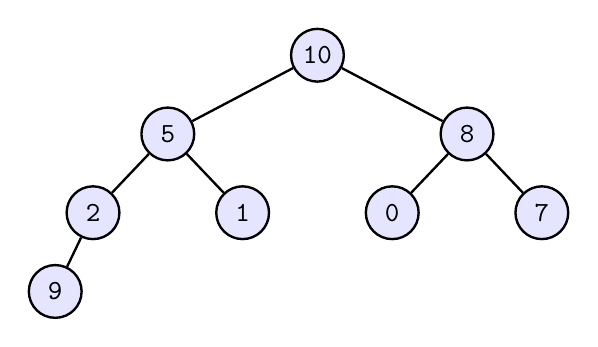
\begin{tikzpicture}

\fill[blue!10] (0.0, 0.0) circle (0.35);
\node [line width=0.03cm,black,minimum size=0.6699999999999999cm,draw,circle] at (0.0,0.0)(10){};\draw (0.0, 0.0) node[color=black] {\texttt{10}};
\fill[blue!10] (-1.9, -1.0) circle (0.35);
\node [line width=0.03cm,black,minimum size=0.6699999999999999cm,draw,circle] at (-1.9,-1.0)(5){};\draw (-1.9, -1.0) node[color=black] {\texttt{5}};
\fill[blue!10] (1.9, -1.0) circle (0.35);
\node [line width=0.03cm,black,minimum size=0.6699999999999999cm,draw,circle] at (1.9,-1.0)(8){};\draw (1.9, -1.0) node[color=black] {\texttt{8}};
\fill[blue!10] (-2.85, -2.0) circle (0.35);
\node [line width=0.03cm,black,minimum size=0.6699999999999999cm,draw,circle] at (-2.85,-2.0)(2){};\draw (-2.85, -2.0) node[color=black] {\texttt{2}};
\fill[blue!10] (-0.95, -2.0) circle (0.35);
\node [line width=0.03cm,black,minimum size=0.6699999999999999cm,draw,circle] at (-0.95,-2.0)(1){};\draw (-0.95, -2.0) node[color=black] {\texttt{1}};
\fill[blue!10] (0.95, -2.0) circle (0.35);
\node [line width=0.03cm,black,minimum size=0.6699999999999999cm,draw,circle] at (0.95,-2.0)(0){};\draw (0.95, -2.0) node[color=black] {\texttt{0}};
\fill[blue!10] (2.85, -2.0) circle (0.35);
\node [line width=0.03cm,black,minimum size=0.6699999999999999cm,draw,circle] at (2.85,-2.0)(7){};\draw (2.85, -2.0) node[color=black] {\texttt{7}};
\fill[blue!10] (-3.33, -3.0) circle (0.35);
\node [line width=0.03cm,black,minimum size=0.6699999999999999cm,draw,circle] at (-3.33,-3.0)(9){};\draw (-3.33, -3.0) node[color=black] {\texttt{9}};\draw[line width=0.03cm,black] (10) to  (5);
\draw[line width=0.03cm,black] (10) to  (8);
\draw[line width=0.03cm,black] (5) to  (2);
\draw[line width=0.03cm,black] (5) to  (1);
\draw[line width=0.03cm,black] (8) to  (0);
\draw[line width=0.03cm,black] (8) to  (7);
\draw[line width=0.03cm,black] (2) to  (9);
\end{tikzpicture}

\end{center}



It's easy to see that in the DFA, the $a$--
and $b$--transitions from the state $\{\}$ goes back to itself.
Therefore the completed DFA is this:


\begin{center}
\begin{tikzpicture}[>=triangle 60,shorten >=0.5pt,node distance=2cm,auto,initial text=, double distance=2pt]
\node[state,initial] (A) at (  0,  0) {$\{q_0\}$};
\node[state] (B) at (  3,  0) {$\{\}$};

\path[->]
(A) edge [bend left=0,pos=0.5,above] node {$a,b$} (B)
(B) edge [loop above] node {$a,b$} ()

;
\end{tikzpicture}
\end{center}
    



\newpage

Solution to Exercise \ref{ex:dfa-as-powerful-as-nfa1}\labeltext{}{sol:dfa-as-powerful-as-nfa1}.

\tinysidebar{\debug{exercises/{dfa-as-powerful-as-nfa1/answer.tex}}}

    Solution not provided.
    

\newpage

Solution to Exercise \ref{ex:dfa-as-powerful-as-nfa2}\labeltext{}{sol:dfa-as-powerful-as-nfa2}.

\tinysidebar{\debug{exercises/{dfa-as-powerful-as-nfa2/answer.tex}}}

    Solution not provided.
    

\newpage

Solution to Exercise \ref{ex:dfa-as-powerful-as-nfa3}\labeltext{}{sol:dfa-as-powerful-as-nfa3}.

\tinysidebar{\debug{exercises/{dfa-as-powerful-as-nfa3/answer.tex}}}

    Solution not provided.
    

\newpage

Solution to Exercise \ref{ex:dfa-as-powerful-as-nfa4}\labeltext{}{sol:dfa-as-powerful-as-nfa4}.

\tinysidebar{\debug{exercises/{dfa-as-powerful-as-nfa4/answer.tex}}}

    Solution not provided.
    

\newpage

Solution to Exercise \ref{ex:closure0}\labeltext{}{sol:closure0}.

\tinysidebar{\debug{exercises/{closure0/answer.tex}}}

    Solution not provided.
    

\newpage

Solution to Exercise \ref{ex:closure1}\labeltext{}{sol:closure1}.

\tinysidebar{\debug{exercises/{closure1/answer.tex}}}

    Solution not provided.
    

\newpage

Solution to Exercise \ref{ex:closure2}\labeltext{}{sol:closure2}.

\tinysidebar{\debug{exercises/{closure2/answer.tex}}}

    Solution not provided.
    

\newpage

Solution to Exercise \ref{ex:closure3}\labeltext{}{sol:closure3}.

\tinysidebar{\debug{exercises/{closure3/answer.tex}}}

    Solution not provided.
    

\newpage

Solution to Exercise \ref{ex:closure4}\labeltext{}{sol:closure4}.

\tinysidebar{\debug{exercises/{closure4/answer.tex}}}

    Solution not provided.
    

\newpage

Solution to Exercise \ref{ex:closure5}\labeltext{}{sol:closure5}.

\tinysidebar{\debug{exercises/{closure5/answer.tex}}}

    Solution not provided.
    

\newpage

Solution to Exercise \ref{ex:closure6}\labeltext{}{sol:closure6}.

\tinysidebar{\debug{exercises/{closure6/answer.tex}}}

    Solution not provided.
    

\newpage

Solution to Exercise \ref{ex:closure7}\labeltext{}{sol:closure7}.

\tinysidebar{\debug{exercises/{closure7/answer.tex}}}

    Solution not provided.
    

\newpage

Solution to Exercise \ref{ex:closure8}\labeltext{}{sol:closure8}.

\tinysidebar{\debug{exercises/{closure8/answer.tex}}}

    Solution not provided.
    

\newpage

Solution to Exercise \ref{ex:closure9}\labeltext{}{sol:closure9}.

\tinysidebar{\debug{exercises/{closure9/answer.tex}}}

    Solution not provided.
    

\newpage

Solution to Exercise \ref{ex:closure10}\labeltext{}{sol:closure10}.

\tinysidebar{\debug{exercises/{closure10/answer.tex}}}

    Solution not provided.
    

\newpage

Solution to Exercise \ref{ex:closure11}\labeltext{}{sol:closure11}.

\tinysidebar{\debug{exercises/{closure11/answer.tex}}}

    Solution not provided.
    

\newpage

Solution to Exercise \ref{ex:closure12}\labeltext{}{sol:closure12}.

\tinysidebar{\debug{exercises/{closure12/answer.tex}}}

    Solution not provided.
    

